\chapter*{\textbf{Практическая часть}}

\section*{\textbf{Функциональная схема разрабатываемой системы на кристале}}

Функциональная схема расзарабатываемой системы на кристале представлена на рисунке \ref{img:func_schema}.

\begin{figure}[H]
	\captionsetup{justification=centering}
	\centering{
		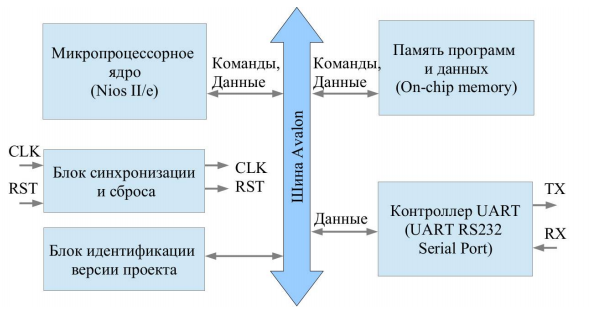
\includegraphics[scale=1]{images/func_schema}
		\caption{Функциональная схема разрабатываемой системы на кристалле}
		\label{img:func_schema}
	}
\end{figure}

Система на кристалле состоит из следующих блоков.

\begin{enumerate}
	\item Микропроцессорное ядро Nios II/e выполняет функции управления
	системой.
	\item Внутренняя оперативная память СНК, используемая для хранения программы
	управления и данных. 
	\item Системная шина Avalon обеспечивает связность всех компонентов системы.
	\item Блок синхронизации и сброса обеспечивает обработку входных сигналов сброса и
	синхронизации и распределение их в системе. Внутренний сигнал сброса
	синхронизирован и имеет необходимую для системы длительность.
	\item Блок идентификации версии проекта обеспечивает хранение и выдачу уникального идентификатора версии, который используется программой управления при инициализации системы.
	\item Контроллер UART обеспечивает прием и передачу информации по
	интерфейсу RS232.
\end{enumerate}
\clearpage

\section*{\textbf{Создание нового модуля системы на кристале QSYS}}


\begin{enumerate}
	\item Был создан новый модуль Qsys.	
	\item Установлена частота внешнего сигнала синхронизации 50 000 000 Гц.
	\item Добавлен в проект модуль синхронизируемого микропроцессорного ядра Nios2.
	\item Добавлен в проект модуль ОЗУ программ и данных.
	\item Добавлены компоненты Avalon System ID, Avalon UART.
	\item Создана сеть синхронизации и сбоса системы.
	\item Сигналы TX и RX экспортированы во внешние порты.
	\item Назначены базовые адреса устройств.
\end{enumerate}

\section*{\textbf{Назначение портами проекта контакты микросхемы}} 

Итог выполненных действий показан на рисунке \ref{img:qsys}.
\begin{figure}[H]
	\captionsetup{justification=centering}
	\centering{
		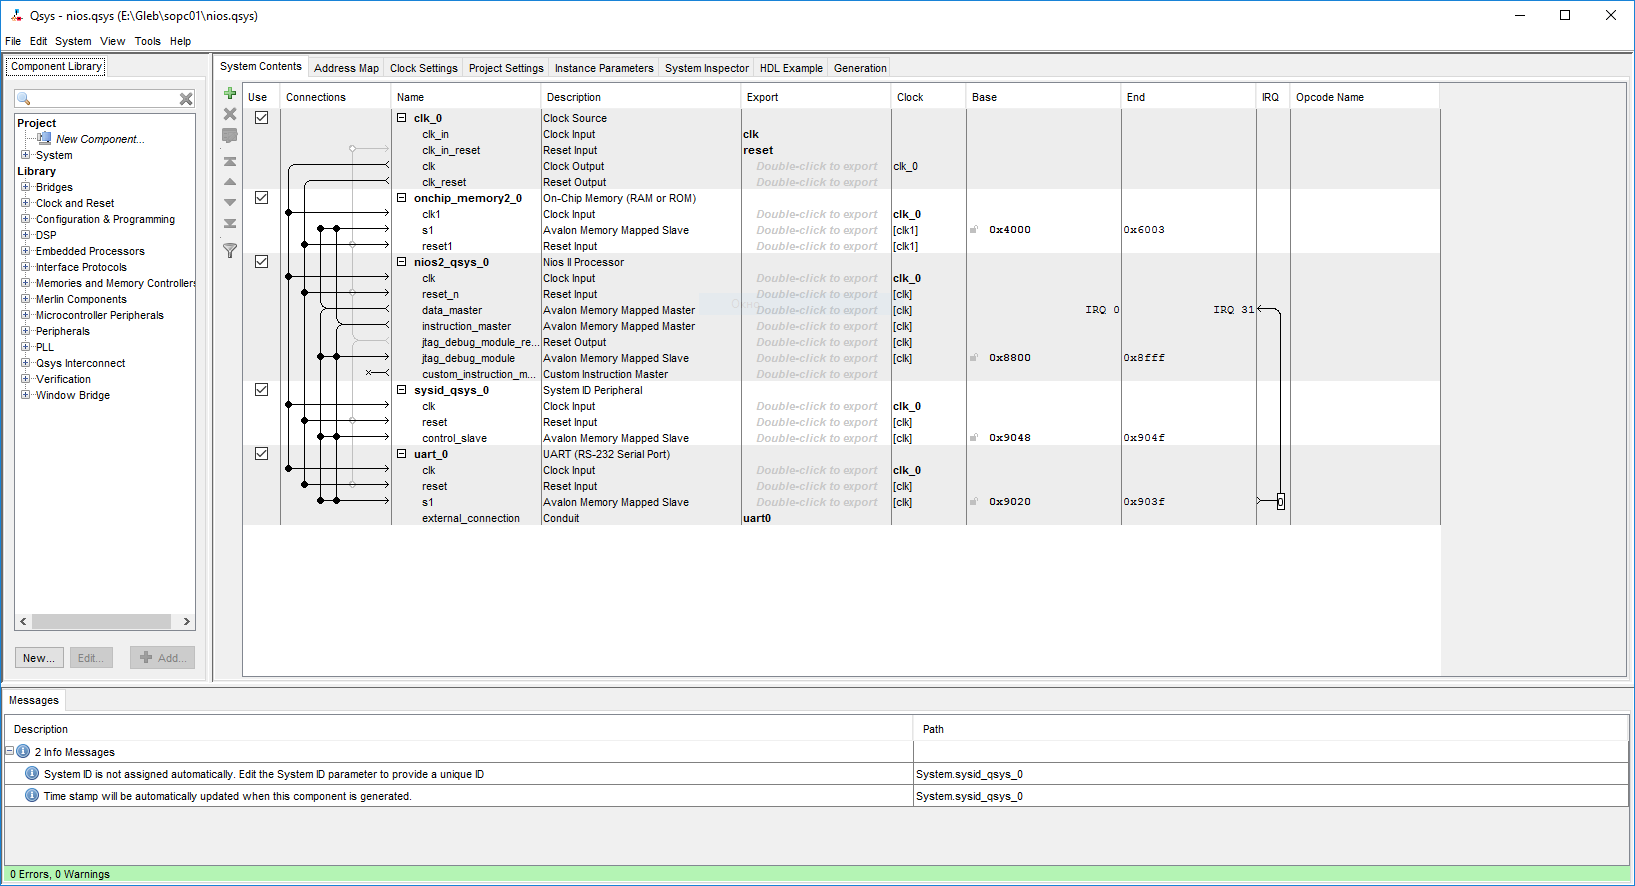
\includegraphics[scale=0.4]{images/ready_module}
		\caption{Готовый модуль в системе проектирования систем на кристалле Altera Qsys}
		\label{img:qsys}
	}
\end{figure}

Назначены контакты в соответствии с таблицей из методических указаний. 

Таблица представлена на рисунке \ref{img:address_table}
\begin{figure}[H]
	\captionsetup{justification=centering}
	\centering{
		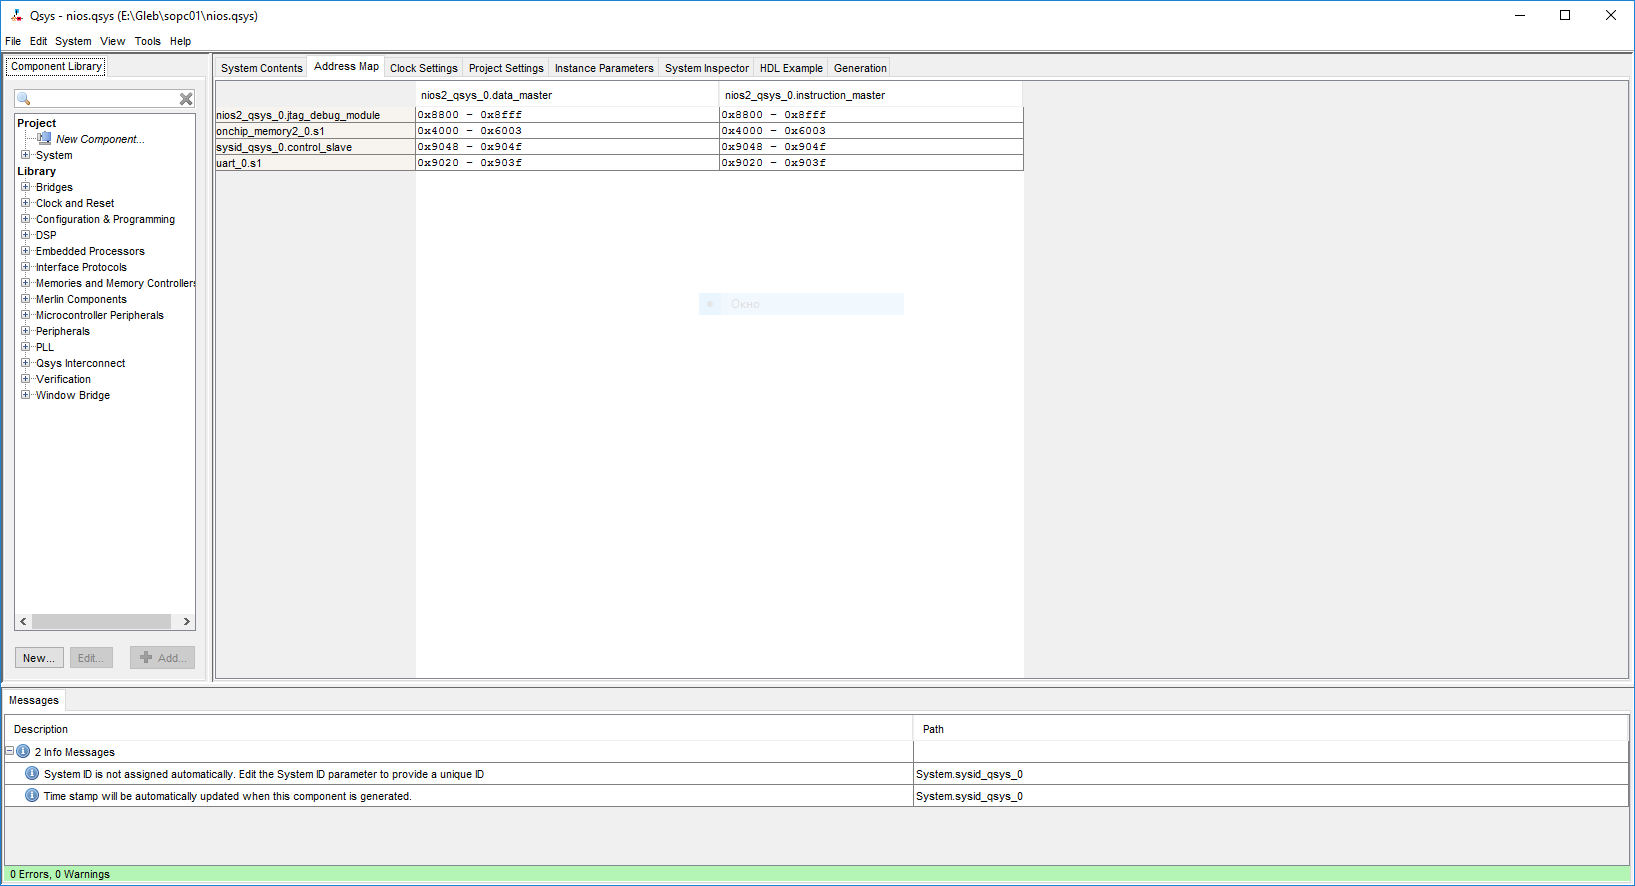
\includegraphics[scale=0.4]{images/address_table}
		\caption{Таблица распределения адресов модулей в системе на кристалле}
		\label{img:address_table}
	}
\end{figure}

\clearpage
Доработанный код проекта представлен на листинге \ref{lst:dop_code} в соответствие с вариантом 16 и группой ИУ7-54Б.
\captionsetup{singlelinecheck = false, justification=raggedright}
\begin{lstlisting}[label=lst:dop_code,caption=Код программного проекта Nios II Software Build Tools for Eclipse]
#include "sys/alt_stdio.h"
#include "system.h"
#include "altera_avalon_sysid_qsys.h"
#include "altera_avalon_sysid_qsys_regs.h"

int main()
{ 
	char ch;
	alt_putstr("Hello from System on Chip\n");
	alt_putstr("Send any character\n");
	
	int id = IORD_ALTERA_AVALON_SYSID_QSYS_ID(SYSID_QSYS_O_BASE);
	char arr[10];
	int i = 0;
	while (i <= 3) {
		arr[3-i] = (char)('0' + id%10);
		id = id/10;
		i = i+1;
	}
	arr[4] = '\0';
	alt_putstr(arr);
	while (1) {
		ch=alt_getchar();
		alt_putchar(ch);
	}
	return 0;
}
\end{lstlisting}
\clearpage

Вывод сообщения с номером варианта и группы представлен на рисунке \ref{img:result}.
\begin{figure}[H]
	\captionsetup{justification=centering}
	\centering{
		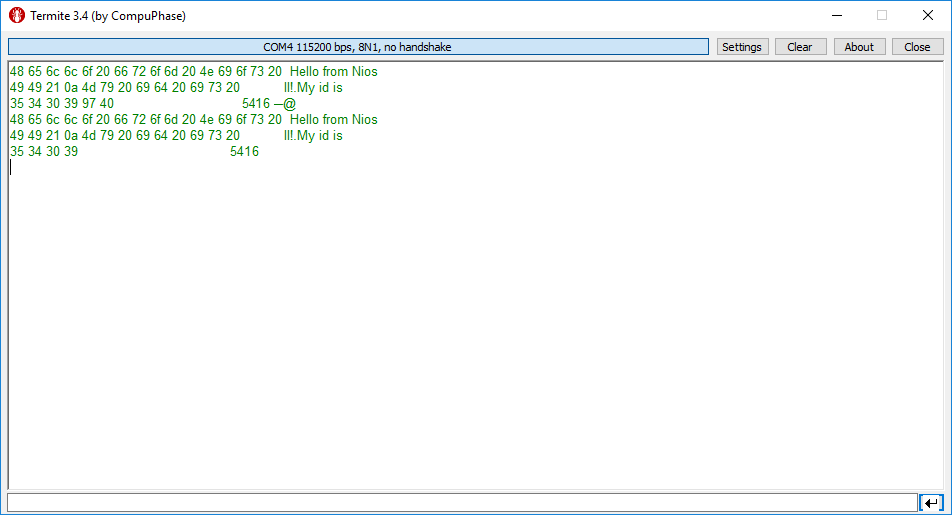
\includegraphics[scale=0.7]{images/result}
		\caption{Результат тестирования PSoC на отладочной плате}
		\label{img:result}
	}
\end{figure}